% Schwingung, angeregt (RLC-Serienschwingkreis mit u_q über C)
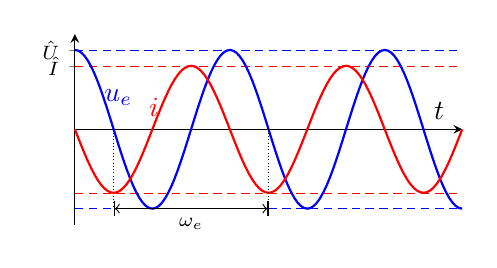
\begin{tikzpicture}[x=1mm,y=1mm] % gilt für tikz-coordinaten außerhalb der axis-environment
    \draw[draw=none] (-6,-2) rectangle (50,25); % Bildrahmen, Koordinatenbezug auf (0,0) des \begin{axis}...\end{axis} pgfplots, für
    \begin{axis}[
        axis lines=center,
        xlabel={$t$},
        x label style={xshift=-3pt},
        xmin=0, xmax=2.5,% 2.5 Periodendauer
        ymin=-1.5, ymax=1.5,
        xtick={\empty},
        xticklabel={\empty},
        xminorticks=false,
        ytick={0,1,1.25},
        yticklabels={,$\scriptstyle{\hat{I}}$,$\scriptstyle{\hat{U}}$},
        yminorticks=false,
        domain=0:2.5,
        samples=121,
        grid=none,
        width=6.5cm,
        height=4.0cm,
        clip=false,
    ]
        \addplot+[mark=none,very thin,blue,densely dashed,] {+1.25};
        \addplot+[mark=none,very thin,blue,densely dashed,] {-1.25};
        \addplot+[mark=none,very thin,red,densely dashed,]  {+1.00};
        \addplot+[mark=none,very thin,red,densely dashed,]  {-1.00};

        \addplot+[mark=none,thick,blue,solid,]   {1.25*sin(x*360+90)};  % u plot
        \addplot+[mark=none,thick,red,solid,]    {-1.0*sin(x*360)};      % i plot

        \node[blue] at (axis cs:0.28,0.5) {$u_e$};
        \node[red] at (axis cs:0.51,0.35) {$i$};

        \addplot+[mark=none,very thin,black,densely dotted,] coordinates {(0.25,-0.0)(0.25,-1.25)};
        \addplot+[mark=none,very thin,black,densely dotted,] coordinates {(1.25,-0.0)(1.25,-1.25)};
        \addplot+[mark=none,black,solid,|<->|] coordinates {(0.25,-1.25)(1.25,-1.25)} node[midway,below] {$\scriptstyle{\omega_e}$};% Tq=2pi/wq
    \end{axis}
\end{tikzpicture}%